\documentclass[10pt]{article}

\def\Type{LessonCaelan}
\def\TypeNum{Lesson 1} %Lesson #
\def\TypeTitle{Slopes \& Rates of Change } %Lesson Title
\def\Semester{Fall 2021} %Not Used 
\def\Course{MATH 1190 \& 1210}%Course number and name
\def\Targets{ \bf\color{ProcessBlue}F1 }

\usepackage{preambleDJ} 

%%%%%%%%%%%% BEGIN DOCUMENT %%%%%%%%%%%%%%%
%%%%%%%%%%%% BEGIN DOCUMENT %%%%%%%%%%%%%%%
%%%%%%%%%%%% BEGIN DOCUMENT %%%%%%%%%%%%%%%
%%%%%%%%%%%% BEGIN DOCUMENT %%%%%%%%%%%%%%%
%%%%%%%%%%%% BEGIN DOCUMENT %%%%%%%%%%%%%%%

\begin{document}
\pagestyle{otherpages}
%\thispagestyle{empty}
\thispagestyle{firstpage}


\vs{0.4}


\textbf{Intended Learning Outcomes}
After this lesson, you will be able to 

\begin{itemize}
    \item Find and distinguish the net change and average rate of change. (\target{F1})
    \item Interpret the average rate of change graphically as the slope the respective linear function. (\target{F1})
\end{itemize}

\vspace{-0.5cm}

\hrulefill

\vspace{0.5cm}


{\bf\color{blue}Warm-up}\exercise \ltrm{\bf\color{ProcessBlue}F1}Respond to the following prompts.\\[-0.25in]
    \begin{enumerate}
    \item[(a)] A predator-prey model describes how the sizes of two populations -- predator $C$ (e.g. Coyotes) and prey $R$ (e.g. Rabbits) -- are related. Suppose two points describing this predator-prey model  are given by $(C_1,R_1)=(100,1000)$ and $(C_2,R_2)=(300,300)$.
        \begin{enumerate}

        \item[i.] What is the net change of the prey population as the predator population changes from $100$ to $300$?\\
             \,\hfill
            %
            {\Large $\Delta R=$\unline{1.5}{} when $C$ changes from\unline{.5}{} to  \unline{.5}{}} 
            %
            \hfill\,\\      
                    \item[ii.] What is the average rate of change of the prey population with respect to the predator population?\\
            
            \,\hfill
            %
            {\Large AROC $=\frac{\Delta R}{\Delta C}=$ \unline{.5}{} }
            %
            \hfill\,\\

        \item[iii.] Assuming the predator-prey model is linear, what is the slope of the graph describing the relationship between the predator and prey populations?

            \,\hfill
            %
            {\Large $m=$\unline{.5}{} }
            %
            \hfill\,\\    
            
        \end{enumerate}
        
    \item[(b)] The equation $F=\dfrac95C+32$ gives the relationship between temperature in degrees Fahrenheit ($F$) and temperature in degrees celsius ($C$). 
        \begin{enumerate}
        \item[i.] What is the slope of the graph describing the relationship between $F$ and $C$?\\
            
            \,\hfill
            %
            {\Large $m=$\unline{.5}{} }
            %
            \hfill\,\\
            
        \item[ii.] What is the (average) rate of change of the temperature in degrees Fahrenheit with respect to the temperature in degrees Celsius?\\
            
            \,\hfill
            %
            {\Large AROC $=\frac{\Delta F}{\Delta C}=$\unline{.5}{} }
            %
            \hfill\,\\

        \item[iii.] What is the net change in the temperature in degrees Fahrenheit when the temperature in degrees Celsius increases by $1$?

            \,\hfill
            %
            {\Large $\Delta F=$\rule[-8pt]{0.5in}{0.4pt} when $\Delta C=$\unline{.5}{} }
            %
            \hfill\,\\
            
        \end{enumerate}
    \end{enumerate}

\newpage
{\bf\color{blue}Discussion.} Based on your recollection of the pre-class activity, how are slope, rate of change, and net change related? Discuss and write down some ideas with your group, and then we will discuss as a class.\\ \vs{-.1}

    \begin{minipage}[t][1.75in]{0.48\textwidth}
    \underline{Group Discussion Notes}
    \end{minipage}
    %
    %\begin{tikzpicture} \draw (0,-5) -- (0,0); \end{tikzpicture} 
    \,\vline \,
    %
    \begin{minipage}[t][1.75in]{0.48\textwidth}
    \underline{Class Discussion Notes}
    \end{minipage}
    %
    \hfill





\begin{minipage}[t]{0.75\textwidth}
\exercise{\bf\color{ProcessBlue}F1} A {\bf demand curve} is a graph depicting the relationship between the price $P$ (per unit) of a certain commodity and the quantity $Q$ units of that commodity that is demanded at that price. The demand curve for a particular commodity is given to the right.

\begin{enumerate}
\item[(a)] What is the {\bf net change} of the price (per unit) of the commodity as the quantity demanded changes from $100$ to $300$ units?
\end{enumerate}

\end{minipage}
%
\hfill
%
\begin{minipage}[t]{0.2\textwidth}
\begin{center}
        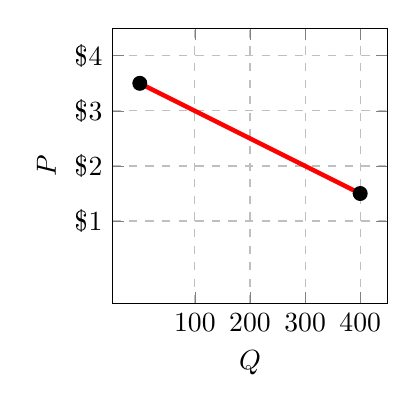
\begin{tikzpicture}[scale=1]
            \begin{axis}[
                %    axis y line = left,
                %    axis x line = bottom,
                    xlabel={$Q$},
                    xtick       = {1,2,3,4},
                    xticklabels = {100,200,300,400},
                    ylabel={$P$},
                    ytick       = {1,2,3,4},
                    yticklabels = {\$1,\$2,\$3,\$4},
                    samples     = 160,
                    domain      = -1:5,
                    restrict y to domain=-1:5,
                    xmin = -0.5, xmax = 4.5,
                    ymin = -0.5, ymax = 4.5,
                    grid=both, grid style=dashed,
                    width=2in, height=2in
                  ]
                  \draw[ultra thick,red] (0,3.5) -- (4,1.5);
                  \filldraw (0,3.5) circle (2.5pt);
                  \filldraw (4,1.5) circle (2.5pt);
            \end{axis}
        \end{tikzpicture}
\end{center}
\end{minipage}

\vfill\vspace{-0.5in}

\begin{enumerate}

\item[(b)] What is the {\bf average rate of change} of the price of $1$ unit of the commodity as the quantity demanded changes from $100$ to $300$ units of the commodity?
    \vfill
\item[(c)] What is the {\bf slope} of the demand curve? What is the {\bf equation} of the demand curve? Be sure to indicate the {\bf domain} - that is, to which values of $Q$ your equation pertains.
    \vfill
    \vfill
\item[(d)] Write a sentence describing what the slope of the demand curve represents in this context.\\ 
({\bf Note:} ``in this context" means your answer must clearly relate to the scenario described in the problem - a demand curve relating a quantity $Q$ and its unit price $P$. Answers like ``rise over run" are not in-context.)
    \vfill
    \vfill
\end{enumerate}

\newpage

\,

\vspace{-0.3in}

\minil {\it Average Rate of Change (AROC) vs. Instantaneous Rate of Change (IROC)}\\

% Average rate of change and instantaneous rate of change answer two different questions. Average rate of change can be used to answer a question like "

\begin{minipage}[t][2.7in]{0.48\textwidth}
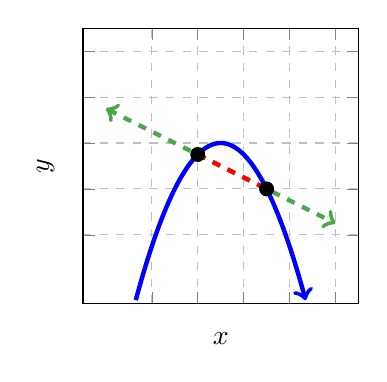
\begin{tikzpicture}[scale=1]
    \begin{axis}[
        %    axis y line = left,
        %    axis x line = bottom,
            xlabel={$x$},
            xtick       = {1,2,3,4,5},
            xticklabels = {},
            ylabel={$y$},
            ytick       = {1,2,3,4,5},
            yticklabels = {},
            samples     = 160,
            domain      = -1:5,
            restrict y to domain=-1:5,
            xmin = -0.5, xmax = 5.5,
            ymin = -0.5, ymax = 5.5,
            grid=both, grid style=dashed,
            width=2in, height=2in
            ]
            % curve
            %\addplot[blue, ultra thick, mark=none, smooth, <->] coordinates{ (0,0) (1,2) (2,3) (3,3) (4,2) (5,.5) };
            \addplot[blue, ultra thick, mark=none, smooth, domain=0.65:4.35, ->] {3-(x-2.5)^2};
            \draw[ultra thick, green!50!black!70, dashed, <->] (0,3.75) -- (5,1.25);
	             \draw[ultra thick, red, dashed] (2,2.75) -- (3.5,2);
	            \filldraw (2,2.75) circle (2.5pt);
	            \filldraw (3.5,2) circle (2.5pt);
    \end{axis}
\end{tikzpicture}
%
\end{minipage}
%
\hfill
%
\vline
%
\hfill
%
\begin{minipage}[t][2.7in]{0.48\textwidth}
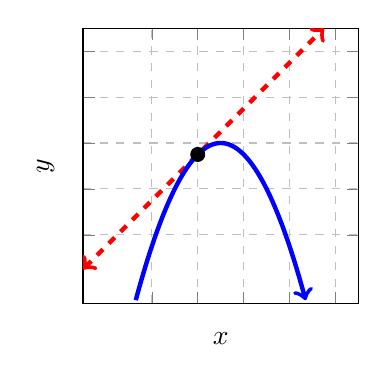
\begin{tikzpicture}[scale=1]
    \begin{axis}[
        %    axis y line = left,
        %    axis x line = bottom,
            xlabel={$x$},
            xtick       = {1,2,3,4,5},
            xticklabels = {},
            ylabel={$y$},
            ytick       = {1,2,3,4,5},
            yticklabels = {},
            samples     = 160,
            domain      = -1:5,
            restrict y to domain=-1:5,
            xmin = -0.5, xmax = 5.5,
            ymin = -0.5, ymax = 5.5,
            grid=both, grid style=dashed,
            width=2in, height=2in
            ]
            % curve
            %\addplot[blue, ultra thick, mark=none, smooth, <->] coordinates{ (0,0) (1,2) (2,3) (3,3) (4,2) (5,.5) };
            \draw[ultra thick, red, dashed, <->] (-0.5,0.25) -- (4.75,5.5);
            \addplot[blue, ultra thick, mark=none, smooth, domain=0.65:4.35, ->] {3-(x-2.5)^2};
            \filldraw (2,2.75) circle (2.5pt);
    \end{axis}
\end{tikzpicture}
%
\end{minipage}

\exercise{\color{ProcessBlue}F1} The graph of $y=3-\left(x-\dfrac52\right)^2$ is given in the mini-lecture above. The instantaneous rate of change of $y$ with respect to $x$ in the instant when $x=2$ is $1$. (We will learn how to compute this quantity directly in a few weeks, but for now let's take it as a given.)

\begin{enumerate}

\item[(a)] Find the average rate of change of $y$ as $x$ changes from $2$ to $4$.{\em Hints:} First sketch  a secant line associated with this quantity  in the coordinate plane below. Second, use the equation above to find $y$ when $x=2$ and  when $x=4$.\\
%
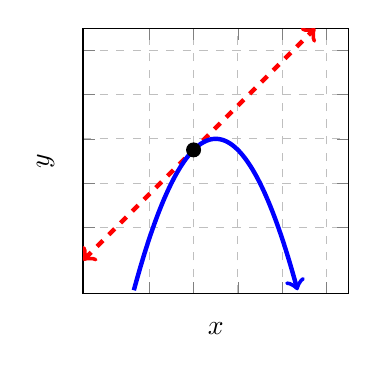
\begin{tikzpicture}[scale=1]
    \begin{axis}[
        %    axis y line = left,
        %    axis x line = bottom,
            xlabel={$x$},
            xtick       = {1,2,3,4,5},
            xticklabels = {},
            ylabel={$y$},
            ytick       = {1,2,3,4,5},
            yticklabels = {},
            samples     = 160,
            domain      = -1:5,
            restrict y to domain=-1:5,
            xmin = -0.5, xmax = 5.5,
            ymin = -0.5, ymax = 5.5,
            grid=both, grid style=dashed,
            width=1.95in, height=1.95in
            ]
            % curve
            %\addplot[blue, ultra thick, mark=none, smooth, <->] coordinates{ (0,0) (1,2) (2,3) (3,3) (4,2) (5,.5) };
             \draw[ultra thick, red, dashed, <->] (-0.5,0.25) -- (4.75,5.5);
            \addplot[blue, ultra thick, mark=none, smooth, domain=0.65:4.35, ->] {3-(x-2.5)^2};
            %\addplot[blue, ultra thick, dashed, mark=none, smooth, domain=2:4.35, ->] {3-(x-2.5)^2};
            \filldraw (2,2.75) circle (2.5pt);
    \end{axis}
\end{tikzpicture}

\item[(b)] Find the average rate of change of $y$ as $x$ changes from $2$ to $3.5$. Then, sketch  a secant line associated with this quantity in the coordinate plane below.\\
%
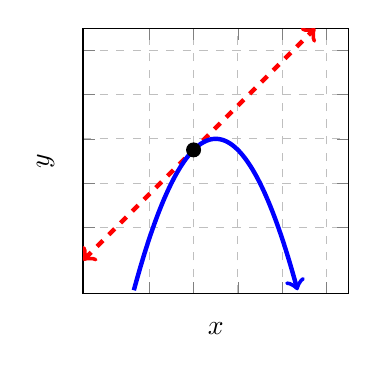
\begin{tikzpicture}[scale=1]
    \begin{axis}[
        %    axis y line = left,
        %    axis x line = bottom,
            xlabel={$x$},
            xtick       = {1,2,3,4,5},
            xticklabels = {},
            ylabel={$y$},
            ytick       = {1,2,3,4,5},
            yticklabels = {},
            samples     = 160,
            domain      = -1:5,
            restrict y to domain=-1:5,
            xmin = -0.5, xmax = 5.5,
            ymin = -0.5, ymax = 5.5,
            grid=both, grid style=dashed,
            width=1.95in, height=1.95in
            ]
            % curve
            %\addplot[blue, ultra thick, mark=none, smooth, <->] coordinates{ (0,0) (1,2) (2,3) (3,3) (4,2) (5,.5) };
             \draw[ultra thick, red, dashed, <->] (-0.5,0.25) -- (4.75,5.5);
            \addplot[blue, ultra thick, mark=none, smooth, domain=0.65:4.35, ->] {3-(x-2.5)^2};
            %\addplot[blue, ultra thick, dashed, mark=none, smooth, domain=2:4.35, ->] {3-(x-2.5)^2};
            \filldraw (2,2.75) circle (2.5pt);
    \end{axis}
\end{tikzpicture}

\item[(c)] Find the average rate of change of $y$ as $x$ changes from $2$ to $2.5$. Then, sketch  a secant line associated with this quantity  in the coordinate plane below.\\
%
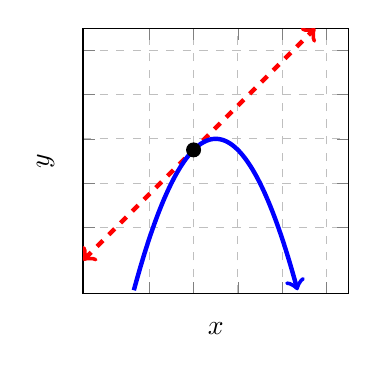
\begin{tikzpicture}[scale=1]
    \begin{axis}[
        %    axis y line = left,
        %    axis x line = bottom,
            xlabel={$x$},
            xtick       = {1,2,3,4,5},
            xticklabels = {},
            ylabel={$y$},
            ytick       = {1,2,3,4,5},
            yticklabels = {},
            samples     = 160,
            domain      = -1:5,
            restrict y to domain=-1:5,
            xmin = -0.5, xmax = 5.5,
            ymin = -0.5, ymax = 5.5,
            grid=both, grid style=dashed,
            width=1.95in, height=1.95in
            ]
            % curve
            %\addplot[blue, ultra thick, mark=none, smooth, <->] coordinates{ (0,0) (1,2) (2,3) (3,3) (4,2) (5,.5) };
             \draw[ultra thick, red, dashed, <->] (-0.5,0.25) -- (4.75,5.5);
            \addplot[blue, ultra thick, mark=none, smooth, domain=0.65:4.35, ->] {3-(x-2.5)^2};
            %\addplot[blue, ultra thick, dashed, mark=none, smooth, domain=2:4.35, ->] {3-(x-2.5)^2};
            \filldraw (2,2.75) circle (2.5pt);
    \end{axis}
\end{tikzpicture}

\hfill {\small\it(part (d) is on the next page $\to$)}

\newpage

\,

\vspace{-0.4in}

\item[(d)] Which of our answers to parts (a), (b), and (c) came the closest to the given instantaneous rate of change of $y$ with respect to $x$ in the instant when $x$ is $2$? How could we have predicted this answer would have been the closest before calculating anything?\\

\vfill
\vfill

\end{enumerate}

{\bf\color{blue} Extra Practice.} \reversemarginpar\marginnote{\fbox{\bf\color{ProcessBlue} F1}} The table below provides a sprinter's approximate position (in meters) from the start line at various times (in seconds) after the start of the 100 meter race.

\begin{center}
    \begin{tabular}{| l | l |}
    \hline
    Time (sec) & Distance (m)\\
    \hline
    8 & 81.7\\
    \hline
    8.3 & 85.6\\
    \hline
    8.5 & 88.2\\
    \hline
    8.8 & 91.3\\
    \hline
    9 & 94.1\\
    \hline
    \end{tabular}
\end{center}

We want to know how fast the sprinter was moving exactly $8.5$ seconds after the beginning of the race. 

\begin{enumerate}
\item[(a)] Evaluate the following quantity {\bf and} describe what the quantity represents in terms of the context given above:
\[ \dfrac{88.2-81.7}{8.5-8} \]

    \vfill
    
\item[(b)]Given the speed of the sprinter is the instantaneous rate of change of position with respect to time, use the data in the table to find 3 different estimates of how fast the sprinter was moving exactly $8.5$ seconds after the beginning of the race.

    \vfill
    \vfill

\item[(c)] Which of your estimates in part (b) is best, and why?

    \vfill

\end{enumerate}

% want them to find slope given a graph, an equation, two points, etc.

% want them to interpret a slope as a rate of change in context

% want them to connect + slope with increasing quantity and - slope with decreasing quantity

% want them to intuit that maximum and minimum values occur where a quantity changes from incr to decr or decr to incr, respectively

\end{document}


%%%%%%%%%%%% F1 Assessment Question %%%%%%%%%%%%%%

\exercise{\bf\color{ProcessBlue}F1} A {\bf supply curve} is a graph depicting the relationship between the quantity $Q$ of a commodity a produce is willing to supply at various prices $P$ of that commodity. The supply curve for a particular commodity is given below.

\begin{center}
        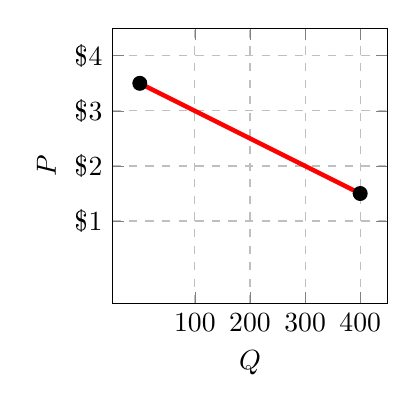
\begin{tikzpicture}[scale=1]
            \begin{axis}[
                %    axis y line = left,
                %    axis x line = bottom,
                    xlabel={$Q$},
                    xtick       = {1,2,3,4},
                    xticklabels = {100,200,300,400},
                    ylabel={$P$},
                    ytick       = {1,2,3,4},
                    yticklabels = {\$1,\$2,\$3,\$4},
                    samples     = 160,
                    domain      = -1:5,
                    restrict y to domain=-1:5,
                    xmin = -0.5, xmax = 4.5,
                    ymin = -0.5, ymax = 4.5,
                    grid=both, grid style=dashed,
                    width=2in, height=2in
                  ]
                  \draw[ultra thick,red] (0,3.5) -- (4,1.5);
                  \filldraw (0,3.5) circle (2.5pt);
                  \filldraw (4,1.5) circle (2.5pt);
            \end{axis}
        \end{tikzpicture}
\end{center}

\begin{enumerate}
\item[(a)] What is the {\bf net change} $\Delta P$ of the price of $1$ unit of the commodity as the quantity supplied changes from $0$ to $300$ units of the commodity?
    \vfill
\item[(b)] What is the {\bf average rate of change} $\dfrac{\Delta P}{\Delta Q}$ of the price of $1$ unit of the commodity as the quantity supplied changes from $0$ to $300$ units of the commodity?
    \vfill
\item[(c)] What is the {\bf slope} of the supply curve? What is the {\bf equation} of the supply curve? Be sure to indicate the {\bf domain} - that is, to which values of $Q$ your equation pertains.
    \vfill
\item[(d)] Write a sentence describing what the slope of the supply curve represents in this context.\\ 
({\bf Note:} ``in this context" means your answer must clearly relate to the scenario described in the problem - a supply curve relating a quantity $Q$ and its unit price $P$. Answers like ``rise over run" are not in this context.)
    \vfill
\end{enumerate}



%%%%%%%%% Unused Exercise %%%%%%%%%

\exercise{\bf\color{ProcessBlue}F1} A {\bf supply curve} is a graph depicting the relationship between the quantity $Q$ of a commodity a produce is willing to supply at various prices $P$ of that commodity. The supply \& demand curves for a particular commodity is given below.

\begin{center}
        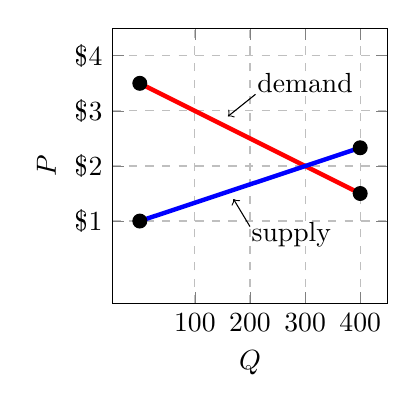
\begin{tikzpicture}[scale=1]
            \begin{axis}[
                %    axis y line = left,
                %    axis x line = bottom,
                    xlabel={$Q$},
                    xtick       = {1,2,3,4},
                    xticklabels = {100,200,300,400},
                    ylabel={$P$},
                    ytick       = {1,2,3,4},
                    yticklabels = {\$1,\$2,\$3,\$4},
                    samples     = 160,
                    domain      = -1:5,
                    restrict y to domain=-1:5,
                    xmin = -0.5, xmax = 4.5,
                    ymin = -0.5, ymax = 4.5,
                    grid=both, grid style=dashed,
                    width=2in, height=2in
                  ]
                  % demand
                  \draw[ultra thick,red] (0,3.5) -- (4,1.5);
                  \filldraw (0,3.5) circle (2.5pt);
                  \filldraw (4,1.5) circle (2.5pt);
                  \node at (3,3.5) {demand};
                  \draw[->] (2.1,3.3) -- (1.6,2.9);
                  % supply
                  \draw[ultra thick, blue] (0,1) -- (4,2.33);
                  \filldraw (0,1) circle (2.5pt);
                  \filldraw (4,2.33) circle (2.5pt);
                  \node at (2.75,.75) {supply};
                  \draw[->] (2,.9) -- (1.7,1.4);
            \end{axis}
        \end{tikzpicture}
\end{center}

\begin{enumerate}
    \item[(a)] Find the slopes of the given supply \& demand curves.

    \begin{center}
    {\Large $m_{\text{supply}}=$\rule[-8pt]{0.5in}{0.4pt} \quad $m_{\text{demand}}=$\rule[-8pt]{0.5in}{0.4pt}}
    \end{center}
    
    \item[(b)] Assuming $P$ is a function of $Q$, we say $P$ is an {\bf increasing} function of $Q$ if $P$ increases as $Q$ increases, and we say $P$ is a {\bf decreasing} function of $Q$ if $P$ decreases as $Q$ increases.\\[0.05in]
    Along the supply curve, is unit price $P$ an increasing or decreasing function of quantity $Q$? Along the demand curve, is unit price $P$ an increasing or decreasing function of quantity $Q$? (circle appropriately below)

    \vspace{-0.3in}

    {\Large
    \begin{align*}
    \text{supply: } &&P \text{ is an} &&\text{increasing} &&/ &&\text{decreasing} &&\text{function of }Q\\[0.1in]
    %
    \text{demand: } &&P \text{ is an} &&\text{increasing} &&/ &&\text{decreasing} &&\text{function of }Q
    \end{align*}
    }

    \item[(c)] How can we decide using only the slopes of the supply \& demand curves whether $P$ is an increasing or decreasing function of $Q$? Explain.

    \vfill

\end{enumerate}